\bigskip
\bigskip
\subsubsection*{Խնդիրներ և հարցեր թեմա 11-ի վերաբերյալ}

\begin{enumerate}[label=\thesection.\arabic*.]

% 12.1
\item Եթե ունենք $(X, \rho)$ մետրիկային տարածություն, ապա ամեն մի ոչ դատարկ $A \subset X$ ենթաբազմության վրա կարելի է սահմանել տոպոլոգիա երկու եղանա\-կով։
\par Առաջին դեպքում դիտարկենք $\rho$ մետրիկի $\left.\rho\right|_A$ սահմանափակումը $A$-ի վրա և վերցնենք $\left.\rho\right|_A$ մետրիկով որոշված $\tau[\left.\rho\right|_A]$ մետրիկային տոպոլոգիան:
\par Երկրորդ դեպքում դիտարկենք $X$-ի $\tau[\rho]$ մետրիկային տոպոլոգիան և վերցնենք նրանով մակածված $\tau[\rho]_A$ տոպոլոգիան $A$-ի վրա:
\par \textbf{Հարց․} Նու՞յնն են արդյոք միշտ $\tau[\left.\rho\right|_A]$ և $\tau[\rho]_A$ տոպոլոգիաները։

\begin{hint}
Պատասխանը գրեթե ակնհայտ դրական է, իսկ ստուգումը կա\-տար\-վում է զուտ սահմանումների մակարդակով։
\end{hint}

% 12.2
\item Նկարագրեք թվային ուղղի սովորական տոպոլոգիայից ամբողջ թվերի $\Z$ են\-թա\-բազ\-մու\-թյան վրա մակածված տոպոլոգիան:

% 12.3
\item Ապացուցեք․ թվային ուղղի ցանկացած երկու
\begin{enumerate}
    \item[ա)] $(a, b)$ և $(c, d)$ տեսքի միջակայքեր սովորական տոպոլոգիայից մակածված տոպոլոգիաներով հոմեոմորֆ տարածություններ են,
    \item[բ)] նույնը $[a, b]$ և $[c, d]$ տեսքի միջակայքերի դեպքում,
    \item[գ)] եթե միջակայքերը տարբեր տեսքերի են՝ մեկը բաց է կամ փակ է, իսկ մյուսը կիսաբաց է, կամ մեկը բաց է, իսկ մյուսը փակ է, ապա ստացված տոպոլոգիական տարածությունները հոմեոմորֆ չեն:
\end{enumerate}

\begin{hint}
Դիտարկեք $f: (a, b) \to (c, d), \ f(x) = c + \dfrac{d-c}{b-a}(x-a)$ ան\-ընդ\-հատ արտապատկերումը և, օգտվելով \hyperref[ch11ex1]{1}, \hyperref[ch11ex2]{2} օրինակներից, կիրառեք \hyperref[ch9thm10]{թեորեմ 10}-ը թեմա 9-ում:
\end{hint}

% 12.4
\item Դիցուք $\R^2$ կոորդինատային հարթությունում ունենք երկու $AB$ և $CD$ հատ\-ված\-ներ: Դիտարկելով այդ հատվածները որպես $\R^2$ տարածության ենթա\-տա\-րա\-ծու\-թյուններ $\R^2$-ից նրանց վրա մակածված տոպոլոգիաներով՝ կառուցեք որևէ $f: AB \to CD$ հոմեոմորֆիզմ:

\begin{hint}
Ներմուծելով $A(x_1, y_1)$, $B(x_2, y_2)$, $C(x_3, y_3)$, $D(x_4, y_4)$ կոոր\-դի\-նատ\-ներ՝ կազմեք $AB$ և $CD$ ուղիղների պարամետրական հավասարումներ նույն $t \in [0, 1]$ տիրույթով և կատարեք պարամետրի արտաքսում։

\par Որոշ դեպքերում պահանջվող հոմեոմորֆիզմը կարելի է կառուցել երկրա\-չա\-փո\-րեն՝ կենտրոնային կամ զուգահեռ պրոյեկտումով, ինչպես ցույց է տրված ստորև օրինակներում:
\end{hint}


\begin{tikzpicture}[
    scale=1.2,
    thick,
    every node/.style={text=black, font=\small},
    dot/.style={circle, fill=black, inner sep=2.0pt} 
]

    % ==========================
    % LEFT FIGURE
    % ==========================
    \begin{scope}[scale=0.8]
        % 1. Define Origin
        \coordinate (O) at (0,0);
        \node[below left] at (O) {$O$};
        \fill (O) circle (1.5pt);

        % 2. Define Rays
        \coordinate (RayTopFar) at (4, 2);
        \coordinate (RayBotFar) at (6, -1);

        % 3. Define Points A, B, C, D
        \coordinate (A) at ($(O)!0.25!(RayBotFar)$);
        \coordinate (C) at ($(O)!0.8!(RayBotFar)$);
        \coordinate (B) at ($(O)!0.55!(RayTopFar)$);
        \coordinate (D) at ($(O)!0.8!(RayTopFar)$);
        
        \coordinate (R) at ($(O)!0.95!(RayBotFar)$);
        \coordinate (Q) at ($(O)!1!(RayTopFar)$);

        % 4. Draw Lines
        \draw (O) -- (Q); 
        \draw (O) -- (R); 
        \draw[blue] (A) -- (B); 
        \draw[blue] (C) -- (D); 

        % 5. Define E 
        % Moved "a bit up" from previous position (0.48 -> 0.65) -> down to 0.55 -> down to 0.45
        \coordinate (E) at ($(A)!0.45!(B)$);
        
        % Calculate f(E) intersection
        \path[name path=LineCD] (C) -- (D);
        \path[name path=RayOE] (O) -- ($(O)!2.5!(E)$);
        \path [name intersections={of=LineCD and RayOE, by=fE}];

        % 6. Draw Ray O -> f(E)
        \draw[dashed] (O) -- (fE);

        % 7. Dots and Labels
        \foreach \p in {A,B,C,D,E,fE} \fill (\p) circle (1.5pt);
        
        \node[below] at (A) {$A$};
        \node[above] at (B) {$B$};
        \node[below] at (C) {$C$};
        \node[above] at (D) {$D$};
        \node[below right, xshift=1pt] at (E) {$E$};
        \node[right, xshift=2pt] at (fE) {$f(E)$};
    \end{scope}


    % ==========================
    % RIGHT FIGURE
    % ==========================
    \begin{scope}[xshift=7.5cm, yshift=-0.75cm, scale=1]
        
        % 1. Define C 
        % Moved "a bit up and left" (Previous: -0.3, 0.7) -> Left to -0.6
        \coordinate (C) at (-0.5, 0.8);

        % 2. Define A relative to C 
        % (Maintains the ~60 degree parallel angle) - AC even smaller (0.6,1.0 -> 0.45, 0.75)
        \coordinate (A) at ($(C) + (0.45, 0.75)$); 

        % 3. Define B relative to A
        % Moved "a tiny bit to the right" (Length increased from 3.0 -> 3.4 -> 3.8)
        \coordinate (B) at ($(A) + (3.4, 0.4)$);

        % 4. Define D on Bottom Line
        % Bottom line passes through C
        \coordinate (BotRef) at (6.0, 0.05); 
        \path[name path=BotLine] (C) -- (BotRef);
        
        % Vector AC for parallel projection
        \coordinate (VecAC) at ($(C)-(A)$);
        
        % Path from B parallel to AC
        \path[name path=LineBD] (B) -- ++(VecAC) -- ++(VecAC); 
        \path [name intersections={of=BotLine and LineBD, by=D}];

        % 5. Define E (on AB)
        % Moved "to the right" (Ratio increased) -> Now "a bit left" (0.45 -> 0.4)
        \coordinate (E) at ($(A)!0.35!(B)$);

        % 6. Calculate f(E)
        \path[name path=LineEfE] (E) -- ++(VecAC) -- ++(VecAC);
        \path [name intersections={of=BotLine and LineEfE, by=fE}];

        % 7. Draw Segments
        % Top: Segment AB
        \draw[blue] (A) -- (B);
        
        % Bottom: Segment CD
        \draw[blue] (C) -- (D);
        
        % Middle Parallel: Ef(E)
        \draw[dashed] (E) -- (fE);
        
        % Left Parallel: AC (Extended top and bottom)
        \draw ($(A)!-1.0!(C)$) -- ($(C)!-1.0!(A)$);
        
        % Right Parallel: BD (Extended top and bottom)
        \draw ($(B)!-0.4!(D)$) -- ($(D)!-0.4!(B)$);

        % 8. Dots and Labels
        \foreach \p in {A,B,C,D,E,fE} \fill (\p) circle (1.5pt);

        \node[above left] at (A) {$A$};
        \node[left] at (C) {$C$};
        \node[right] at (B) {$B$};
        \node[below right] at (D) {$D$};
        \node[above right, yshift=2pt] at (E) {$E$};
        \node[below, xshift=-2pt] at (fE) {$f(E)$};

    \end{scope}

\end{tikzpicture}

% 12.5
\item Ստորև պատկերված են ա) շրջանագիծ, բ) օվալ (ինքն իրեն չհատող փակ գիծ), գ) բազմանկյուն՝ որպես էվկլիդյան հարթության ենթատարածություն\-ներ, և ինքն իրեն չհատող երեքնուկաձև փակ գիծը՝ որպես եռաչափ տարածու\-թյան ենթատարածություն:

\begin{center}
\begin{tikzpicture}[
    scale=1,
    line width=1pt,
    color=black,
    % Style for English labels
    label text/.style={anchor=north, yshift=-0.5cm}
]

    % ==========================
    % Figure a: Circle
    % ==========================
    \begin{scope}[xshift=0cm]
        \draw (0,-0.05) circle (1.05cm);
        \node[label text] at (0,-1.1) {(ա)};
    \end{scope}

    % ==========================
    % Figure b: The "C" Shape
    % ==========================
    \begin{scope}[xshift=3.5cm, yscale=-0.029, xscale=0.029, yshift=0.1cm]
        \draw
(4.75,-26.5)
.. controls (21.75,-1.5) and (2.75,0.5) ..
(-2.25,-18.5)
.. controls (-7.25,-37.5) and (-46.25,-3.5) ..
(-13.25,22.5)
.. controls (19.75,48.5) and (14.75,-2.5) ..
(32.75,2.5)
.. controls (50.75,7.5) and (22.75,59.5) ..
(-19.25,28.5)
.. controls (-61.25,-2.5) and (-12.25,-51.5) ..
(4.75,-26.5)
-- cycle;
        \node[label text] at (0,-1.1/-0.029) {(բ)};
    \end{scope}

    % ==========================
    % Figure c: The Polygon
    % ==========================
    \begin{scope}[xshift=7cm, yshift=-0.15cm, scale=0.7]
        \draw
        (-2,0)
        -- (-1,1.6)
        -- (-0.1,0.2)
        -- (2,1.2)
        -- (0.5,-0.4)
        -- (1.2,-1.2)
        -- (-0.7,-1.4)
        -- cycle;
        \node[label text] at (0,-1.1/0.7+0.15/0.7) {(գ)};
    \end{scope}

    % ==========================
    % Figure d: Perfect Trefoil Knot (Better Over/Under)
    % ==========================
    \begin{scope}[xshift=10.5cm, scale=-0.415, yshift=-0.3cm] % Scaled up slightly (0.35 -> 0.4) and moved down (1.0 -> 0.5)
        % Parametric Equations for Trefoil:
        % x = sin(t) + 2 sin(2t)
        % y = cos(t) - 2 cos(2t)
        % Domain 0 to 360 covers the whole knot.
        % Rotated/flipped by using negative signs as before to orient loop up.

        % 1. Draw the FULL knot first as the "background"
        \draw plot[domain=0:360, samples=90, smooth] 
            ({-(sin(\x) + 2*sin(2*\x))}, {-(cos(\x) - 2*cos(2*\x))});

        % 2. Draw "Over" segments with a double-line effect
        % We draw a thick WHITE line first (to erase the crossing underneath),
        % then the black line again on top.
        
        % Crossing 1 (Bottom Right):
        % Parametric range approx 90-110 crosses over approx 330-350
        \draw[line width=4.5pt, color=white] plot[domain=90:110, samples=20, smooth] 
             ({-(sin(\x) + 2*sin(2*\x))}, {-(cos(\x) - 2*cos(2*\x))});
        \draw plot[domain=90:110, samples=20, smooth] 
             ({-(sin(\x) + 2*sin(2*\x))}, {-(cos(\x) - 2*cos(2*\x))});

        % Crossing 2 (Top Center):
        % Parametric range approx 210-230 crosses over approx 90-110 logic? 
        % Actually checking the symmetry: 210-230 is the top loop crossing over.
        \draw[line width=4.5pt, color=white] plot[domain=210:230, samples=20, smooth] 
             ({-(sin(\x) + 2*sin(2*\x))}, {-(cos(\x) - 2*cos(2*\x))});
        \draw plot[domain=210:230, samples=20, smooth] 
             ({-(sin(\x) + 2*sin(2*\x))}, {-(cos(\x) - 2*cos(2*\x))});

        % Crossing 3 (Bottom Left):
        % Parametric range approx 330-350 crosses over.
        \draw[line width=4.5pt, color=white] plot[domain=330:350, samples=20, smooth] 
             ({-(sin(\x) + 2*sin(2*\x))}, {-(cos(\x) - 2*cos(2*\x))});
        \draw plot[domain=330:350, samples=20, smooth] 
             ({-(sin(\x) + 2*sin(2*\x))}, {-(cos(\x) - 2*cos(2*\x))});

        % Label position adjusted to align with others
        % We want the label to appear at approximately the same visual height.
        % Others are at y = -1.1. 
        % Here we are scaled by 0.4 and shifted by 0.5.
        % To match visual y=-1.1 relative to the baseline of other figures:
        \node[label text] at (0,3) {(դ)}; 
    \end{scope}

\end{tikzpicture}
\end{center}

\par Ապացուցեք, որ դրանք հոմեոմորֆ են իրար:

\begin{hint}
Շրջանագծի վրա վերցրեք $A_1$, $A_2$, $\dots$, $A_6$ կետեր, «երեքնուկի» վրա՝ $B_1$, $B_2$, $\dots$, $B_6$ կետեր։

\begin{center}
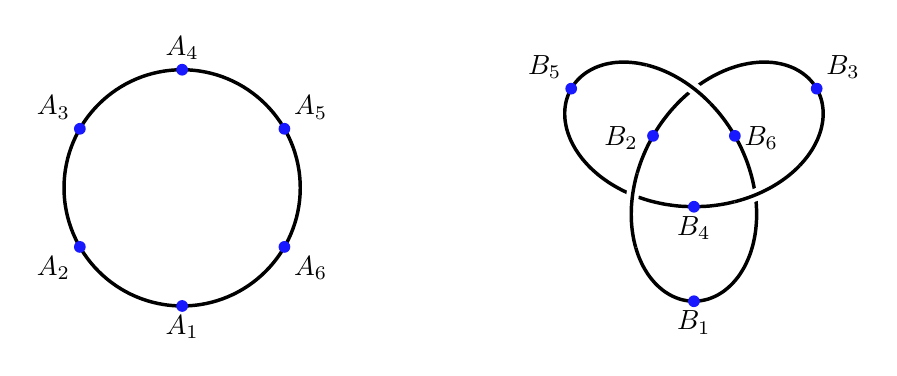
\begin{tikzpicture}[
    scale=1.0,
    every node/.style={text=black},
    dot/.style={circle, fill=blue!90, inner sep=1.5pt}
]

    % ==========================
    % LEFT FIGURE: The Circle
    % ==========================
    \begin{scope}[xshift=0cm]
        \draw[line width=1.25pt, black] (0,0) circle (1.5cm);

        % Brace the position values to prevent 'unknown key' error
        \foreach \i/\angle/\pos in {
            1/270/below, 
            2/210/{below left}, 
            3/150/{above left}, 
            4/90/above, 
            5/30/{above right}, 
            6/-30/{below right}} 
        {
            \node[dot] (A\i) at (\angle:1.5cm) {};
            \node[\pos] at (A\i) {$A_{\i}$};
        }
    \end{scope}


    % ==========================
    % RIGHT FIGURE: The Trefoil Knot
    % ==========================
    \begin{scope}[xshift=6.5cm, scale=0.6, yshift=0.6cm] 
        
        % NOTE: Removed the negative sign from Y coordinate to flip the shape
        % vertically so it points DOWN (matching your B1 at bottom sketch).
        
        % 1. Draw the FULL knot (Background)
        \draw[line width=1.25pt, color=black] plot[domain=0:360, samples=100, smooth] 
            ({-(sin(\x) + 2*sin(2*\x))}, {(cos(\x) - 2*cos(2*\x))});

        % 2. Draw "Over" segments (Halo Effect)
        
        % Crossing 1 (Bottom Right area in this orientation)
        \draw[line width=4.5pt, color=white] plot[domain=90:110, samples=20, smooth] 
             ({-(sin(\x) + 2*sin(2*\x))}, {(cos(\x) - 2*cos(2*\x))});
        \draw[line width=1.25pt, color=black] plot[domain=90:110, samples=20, smooth] 
             ({-(sin(\x) + 2*sin(2*\x))}, {(cos(\x) - 2*cos(2*\x))});

        % Crossing 2 (Top Center area)
        \draw[line width=4.5pt, color=white] plot[domain=210:230, samples=20, smooth] 
             ({-(sin(\x) + 2*sin(2*\x))}, {(cos(\x) - 2*cos(2*\x))});
        \draw[line width=1.25pt, color=black] plot[domain=210:230, samples=20, smooth] 
             ({-(sin(\x) + 2*sin(2*\x))}, {(cos(\x) - 2*cos(2*\x))});

        % Crossing 3 (Bottom Left area)
        \draw[line width=4.5pt, color=white] plot[domain=330:350, samples=20, smooth] 
             ({-(sin(\x) + 2*sin(2*\x))}, {(cos(\x) - 2*cos(2*\x))});
        \draw[line width=1.25pt, color=black] plot[domain=330:350, samples=20, smooth] 
             ({-(sin(\x) + 2*sin(2*\x))}, {(cos(\x) - 2*cos(2*\x))});

        % 3. Place Labels B1...B6
        % Adjusted angles for the flipped (Point Down) orientation
        \foreach \i/\t/\pos in {
            1/180/below,        
            2/240/{below left, yshift=7pt, xshift=-2pt}, 
            3/300/{above right, yshift=0pt}, 
            4/0/below,          
            5/60/{above left, yshift=0pt}, 
            6/120/{below right, yshift=7pt}} 
        {
            % Calculate coordinate
            \pgfmathsetmacro{\px}{-(sin(\t) + 2*sin(2*\t))}
            \pgfmathsetmacro{\py}{(cos(\t) - 2*cos(2*\t))} % Removed minus here too
            
            \node[dot] (B\i) at (\px,\py) {};
            \expandafter\node\expandafter[\pos] at (B\i) {$B_{\i}$};
        }
        
    \end{scope}

\end{tikzpicture}
\end{center}

\par Ընտրելով $f_i: A_i A_{i+1} \to B_i B_{i+1},\ i=1, 2, \dots, 5$ և $f_6: A_6 A_1 \to B_6 B_1$ հոմե\-ո\-մոր\-ֆիզմներ՝ կառուցեք հոմեոմորֆիզմ շրջանագծի և «երեքնուկի» միջև օգտվե\-լով \hyperref[ch11thm3]{թեորեմ 3}-ից:
\end{hint}

% 12.6
\item Դիտարկենք թվային ուղղի $(-1, 1)$ ենթաբազմությունը նրա վրա սովո\-րա\-կան տոպոլոգիայից մակածված տոպոլոգիայով։ Ապացուցեք, որ այդ տա\-րա\-ծու\-թյու\-նը հոմեոմորֆ է $(\R, \text{սովոր․})$ տարածությանը։

\begin{hint}
Օգտվեք թեմա 1-ի \hyperref[ch1ex9]{օրինակ 9}-ում բերված արտապատկերումից։
\end{hint}

\par Ստորև 12.7-12.10 խնդիրներում կորերը և մակերևույթները դիտարկվում են հա\-մա\-պա\-տաս\-խա\-նա\-բար $(\R^2, \text{սովոր․})$ և $(\R^3, \text{սովոր․})$ տարածություններից մա\-կ\-ած\-ված տոպոլոգիաներով։ Ապացուցեք․

% 12.7
\item ցանկացած պարաբոլ հոմեոմորֆ է ուղղի;

% 12.8
\item ցանկացած միախոռոչ հիպերբոլոիդ հոմեոմորֆ է ուղիղ շրջանային գլանի;

% 12.9
\item ցանկացած երկխոռոչ հիպերբոլոիդ հոմեոմորֆ է հարթությունների զույգի;

% 12.10
\item ցանկացած էլիպսական պարաբոլոիդ հոմեոմորֆ է հարթության։

% 12.11
\item Ապացուցեք․ հաշվելիության առաջին և երկրորդ աքսիոմները ժառանգական հատկություններ են: Այսինքն՝ եթե որևէ տարածություն բավարարում է առա\-ջին (երկրորդ) աքսիոմին, ապա նրա ցանկացած ենթատարածություն նույն\-պես բավարարում է այդ նույն աքսիոմին։
\end{enumerate}
